\documentclass[10pt, oneside]{article}   	% use "amsart" instead of "article" for AMSLaTeX format
\usepackage{geometry}                		% See geometry.pdf to learn the layout options. There are lots.
\geometry{letterpaper}                   		% ... or a4paper or a5paper or ... 
%\geometry{landscape}                		% Activate for for rotated page geometry
%\usepackage[parfill]{parskip}    		% Activate to begin paragraphs with an empty line rather than an indent
\usepackage{graphicx}				% Use pdf, png, jpg, or eps§ with pdflatex; use eps in DVI mode
								% TeX will automatically convert eps --> pdf in pdflatex		
\usepackage{amsmath, amssymb}    % May not all be necessary
\usepackage{graphicx}                    % For including pictures
\usepackage{hyperref}                    % For formatting (clickable) URLs
\usepackage{algpseudocode}
\usepackage{algorithm}
\usepackage{mfirstuc}
\usepackage{graphicx}
\usepackage{amsopn}
\usepackage{url}
\usepackage{parskip}
\usepackage{wrapfig}
\usepackage{color}
\usepackage[usenames,dvipsnames,svgnames,table]{xcolor}
\usepackage{grffile}
\usepackage{comment}
\usepackage{epsfig}
\usepackage{float}
\usepackage{subfigure}
\usepackage{verbatim}
\usepackage{multirow}
\usepackage{todonotes}
\usepackage{epstopdf}
\usepackage{amssymb}
\usepackage{multirow}
\usepackage{hhline}

\presetkeys{todonotes}{inline}{}

\newcommand\figref{Fig.~\ref}
\newcommand\secref{Section~\ref}
\newcommand\tabref{Table~\ref}

\title{CS 659 Course Project: Restaurant Revenue Prediction}
\author{Huangxin Wang and Zhonghua Xi \\
\\
Computer Science Dept. George Mason University}
%\date{}							% Activate to display a given date or no date

\begin{document}
\maketitle

\begin{abstract}
In this project, we work on predicting revenue for restaurants which is a competition hosted in Kaggle. The dataset provided by TFI contains a training set of  $137$ restaurants records, and a test set of $100, 000$  restaurants records. We pre-process data to handle with categorical data and missing value. We explore the dataset by studying the correlation between features, feature ranking and principal component analysis. We test different models including GradientBoostingRegressor, svm.NuSVR, KNeighborsRegressor, RandomForestRegressor and so on. We find that an ensemble of a subset of these prediction models perform the best than a single model. Using RMSE evaluation approach, our prediction models is ranked within top $10\%$ of all participated teams in the competition.
\end{abstract}

\section{Introduction}
\todo{re-phrase this section}
Deciding when and where to open new restaurants is largely a subjective process based on the personal judgement and experience of development teams. 
This subjective data is difficult to accurately extrapolate across geographies and cultures.
New restaurant sites take large investments of time and capital to get up and running. 
When the wrong location for a restaurant brand is chosen, the site closes within 18 months and operating losses are incurred. 
Finding a mathematical model to increase the effectiveness of investments in new restaurant sites would allow funds to invest more in other important business areas, like sustainability, innovation, and training for new employees.
The goal of this project is to predict the revenues of restaurants by given demographic, real estate, and commercial data of existing restaurants withe their current revenues.

%\subsection{}
\section{Data Analysis and Processing}
The dataset is from Kaggle, a community of data scientists which also hosts data science competitions. 
Restaurant revenue prediction is one of the active competition.
There are 137 restaurants in the training set and 100000 in the test set which is an unbalanced dataset. 
For each record, 41 features are given detailed in \tabref{tab:features}.

\begin{table}[htdp]
\footnotesize
\caption{Features}
\begin{center}
\begin{tabular}{|r|l|}
\hline
\bf{Name} 		& \bf{Description} \\ \hline
\bf{Open Date}	& Categorical. Opening date for a restaurant. \\ \hline
\bf{City}		& Categorical. City that the restaurant is in. \\ \hline
\bf{City Group} & Categorical. Type of the city. Big cities, or Other. \\ \hline
\bf{Type}		& \begin{tabular}{@{}l@{}} Categorical. Type of the restaurant. \\ FC: Food Court, IL: Inline, DT: Drive Thru, MB: Mobile. \end{tabular}   \\ \hline
\bf{P1-P37}		& \begin{tabular}{@{}l@{}} Numerical. Three categories of these obfuscated data. \\ 
\bf{Demographic data} \\
Gathered from third party providers with GIS systems. \\ 
These include population in any given area, age and \\
gender distribution, development scales. \\
\bf{Real estate data} \\
Mainly relate to the m2 of the location, front facade \\
of the location, car park availability. \\
\bf{Commercial data} \\
Mainly include the existence of points of interest \\
including schools, banks, other QSR operators. \end{tabular}   \\ \hline
\bf{Revenue}	& \begin{tabular}{@{}l@{}} A transformed revenue of the restaurant in a given year \\
Only provided in training set.
\end{tabular} \\ \hline
\end{tabular}
\end{center}
\label{tab:features}
\end{table}%

\subsection{Evaluation}
\subsubsection{What to submit?}
For each records in the test set, output the ID of that record followed by the predicted revenue.

\subsubsection{Evaluation Metric}
Submissions are scored on the root mean squared error. 
RMSE is very common and is a suitable general-purpose error metric. 
Compared to the Mean Absolute Error, RMSE punishes large errors:
\begin{equation*}
RMSE = \sqrt{\frac{1}{n} \sum_{i=1}^{n} (y_i - \hat{y}_i)^2 }, 
\end{equation*}
where $\hat{y}_i$ is the predicted revenue and $y_i$ is the ground truth.

\subsubsection{Public Board V.S. Private Board}
For an active competition, each submission will be evaluated only on the 30\% of test set and scores will be published on the public board.
Once the competition is over, the final score is evaluated on the rest 70\% of the test set which will be published on the private board. 
Who win the public board may not win the private board since his model may be overfitted the public board's test data.
   
\subsection{Data Preparation}
\subsubsection{Revenue at a Glance}
In \figref{fig:revenue} we show the histogram of the revenues in the training set, from which we can see that majority of the revenues are around $5 \times 10^6$, 
however, there are few ``outliers'' which makes both training and prediction hard especially under RMSE evaluation metric.

\begin{figure}[htbp] %  figure placement: here, top, bottom, or page
   \centering
   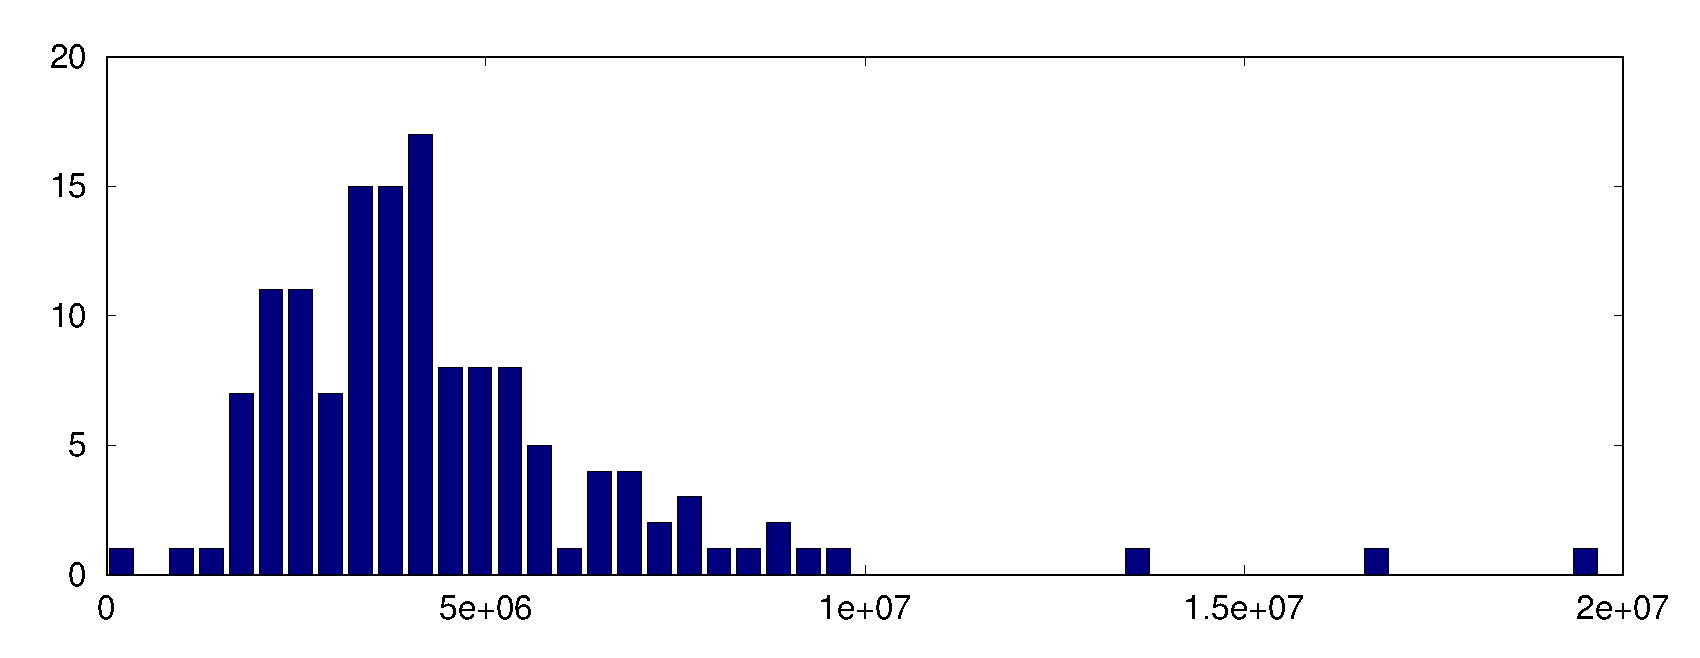
\includegraphics[width=5in]{figs/revenue.eps} 
   \caption{Histogram of revenues.}
   \label{fig:revenue}
\end{figure}

\subsubsection{Features Selection}

{\bf Missing Categories} 
After a quick exploration of both training set and test set we found that both {\bf City} and {\bf Type} features have unseen categories in the training set.
There are total 63 cities in the entire dataset, too many new features will be added if we create a binary feature for each city and 
the there is no correlation between these two features and revenue.
Thus we decided to drop both {\bf City} and {\bf Type} features.

{\bf Feature Rank}
We use feature \textbf{Select attributes} to rank features. In specific, we use attribute evaluator \textbf{ReliefAttributeEval} with search method \textbf{Ranker}, the cross validation is set as 5 folds. ReliefAttributeEval is an attribute evaluator that evaluates the worth of an attribute by repeatedly sampling an instance and considering the value of the given attribute for the nearest instance of the same and different class. It can operate on both discrete and continuous class data. We get the following feature rank results


{\scriptsize
\begin{verbatim}
=== Attribute selection 5 fold cross-validation seed: 10 ===

average merit      average rank  attribute
 0.02  +- 0.007      1   +- 0        1 Open Date
 0.002 +- 0.002      5.2 +- 2.93    17 P13
 0.003 +- 0.005      5.8 +- 4.21    33 P29
 0.001 +- 0.003      6.6 +- 2.15    16 P12
-0.001 +- 0.005      7   +- 4.65    21 P17
 0.002 +- 0.004      7.2 +- 5.78    25 P21
 0     +- 0.002      7.4 +- 3.5     14 P10
 0     +- 0.001      7.6 +- 4.27    12 P8
-0.002 +- 0.004      9.4 +- 4.22    32 P28
-0.001 +- 0.002      9.6 +- 6.25     8 P4
-0.003 +- 0.004     10.2 +- 3.12    40 P36
-0.003 +- 0.003     10.8 +- 2.56    22 P18
-0.005 +- 0.004     14   +- 3.03    38 P34
-0.005 +- 0.003     15   +- 3.46    13 P9
-0.006 +- 0.003     16.4 +- 5.35    26 P22
-0.006 +- 0.004     16.6 +- 5.68    10 P6
-0.008 +- 0.006     18.8 +- 5.67    29 P25
-0.008 +- 0.004     19.2 +-10.17    15 P11
-0.008 +- 0.005     19.6 +- 2.73     5 P1
-0.008 +- 0.004     20   +- 5.93     7 P3
-0.009 +- 0.005     21.2 +- 1.6     20 P16
-0.009 +- 0.004     21.4 +- 7.94     9 P5
-0.011 +- 0.006     23.4 +- 8.69    24 P20
-0.011 +- 0.005     23.6 +- 3.72    18 P14
-0.011 +- 0.004     23.8 +- 2.32    39 P35
-0.011 +- 0.005     24.6 +- 2.94    36 P32
-0.012 +- 0.003     26.2 +- 3.66    27 P23
-0.014 +- 0.006     28   +- 4.15    30 P26
-0.015 +- 0.004     28.4 +- 5.57     4 Type
-0.015 +- 0.006     28.6 +- 5.54    34 P30
-0.015 +- 0.007     29.6 +- 3.93    37 P33
-0.016 +- 0.006     32.4 +- 4.08    35 P31
-0.016 +- 0.005     32.6 +- 3.01    31 P27
-0.017 +- 0.007     33.4 +- 3.98    28 P24
-0.017 +- 0.004     34   +- 2.61    11 P7
-0.019 +- 0.007     34.2 +- 3.19    41 P37
-0.018 +- 0.006     34.2 +- 2.23    19 P15
-0.018 +- 0.004     34.6 +- 2.87    23 P19
-0.026 +- 0.004     38.4 +- 0.8      6 P2
-0.038 +- 0.004     40.2 +- 0.4      3 City Group
-0.04  +- 0.005     40.8 +- 0.4      2 City
 \end{verbatim}
}


\subsection{Principal Component Analysis (PCA)} We apply principal component analysis after cleaning the data (i.e., transform open data and categorical data to numeric data). Principal components analysis is useful in reducing dimensionality by choosing enough eigenvectors to account for some percentage of the variance of in the original data. Here we set the variance as $95\%$. We conduct principal components on both the training dataset, testing dataset, and the combination of training and testing dataset. The results are presented in Figure~\ref{fig:pca_train} and Figure~\ref{fig:pca_test} and Figure~\ref{fig:pca_all} respectively. From the figure, we can see the $15$ attributes are required to cover $95\%$ variance of the training set, while $35$ attributes are required to cover the $95\%$ of testing dataset, or the combination of training and testing dataset.

\begin{figure}[!ht] %  figure placement: here, top, bottom, or page
   \centering
   \includegraphics[width=5in]{figs/pca_seperate.PNG} 
   \caption{Principal Components Analysis on the training dataset}
   \label{fig:pca_train}
\end{figure}

\begin{figure}[!ht] %  figure placement: here, top, bottom, or page
   \centering
   \includegraphics[width=5in]{figs/pca_test.PNG} 
   \caption{Principal Components Analysis on the testing dataset}
   \label{fig:pca_test}
\end{figure}

\begin{figure}[htbp] %  figure placement: here, top, bottom, or page
   \centering
   \includegraphics[width=5in]{figs/pca_all.PNG} 
   \caption{Principal Components Analysis on the complete dataset, including training and testing data.}
   \label{fig:pca_all}
\end{figure}

\subsubsection{Feature Normalization}
Since features have different scale and ranges, feature normalization is a necessary preprocessing step if we would like to compute the distance between two instances which is used for finding nearest neighbors. 
For example, one feature ranges from 1 to 1000 will dominant the distance computation if all other features are range from 0 to 1.
We choose to use standardization on the entire dataset (stack training set and test set together) such that each feature is transformed to zero mean and unit variance.

\section{Results and Discussion}

\subsection{Toolbox}
We use Scikit-Learn which is a open source python library built on NumPy, SciPy, and matplotlib. 
It provides simple and efficient tools for data mining and data analysis range from Classification, Regression, Clustering, Dimensionality reduction, Model selection and Preprocessing.

\subsection{Single Model Selection}
We start from single model, model selection is done based on the average error of a 3 folds cross-validation.
Models with their best cross-validation scores and the parameters are shown in \tabref{tab:single_model}, and we evaluated them on the public board.
From \tabref{tab:single_model} we can see, with a well-tuned single model, we can only beat about half of the teams.
The next step is to ensemble those single models.

\begin{table}[htdp]
\caption{Single Model Performance}
\begin{center}
\begin{tabular}{|c|c|c|c|l|}
\hline 
Model & CV ($10^6$)  & PB ($10^6$)  & Rank & Parameters \\ \hline 
KNN & 2.30149 &   1.76177 & 1050 &  n-neighbors=22, weights=`distance' \\ \hline 
NuSVR & 2.30379 &   1.73142 & 829 &  nu=0.38, C=1.8547e6, gamma=0.004 \\ \hline 
GB  & 2.33207 &   1.80864 &  1361 & \begin{tabular}{@{}l@{}} n-estimators=100, learning-rate=0.1, \\ max-depth=3, loss=`lad', subsample=0.95 \end{tabular} \\ \hline
SVR	& 2.32837 &	1.90432 	& 1792 & 	C=1.8547e6, epsilon=0.0001, gamma=0.02 \\ \hline
RF	& 2.35433 &	1.80236 	& 1321	 & n-estimators=100, min-weight-fraction-leaf=0.1 \\ \hline
\end{tabular}
\\
{\small GB = GradientBoostingRegressor. RF = RandomForestRegressor. \\ CV = Cross-validation score. PB = Public board score.}
\end{center}
\label{tab:single_model}
\end{table}%

\subsection{Ensamble}
Model ensemble is widely adopted especially in Kaggle competitions in the cases that scores can not be improved any further by using a single model.
We ensemble 3 models, final prediction is a linear combination (weighted average) of the predictions from all the models.
Parameters and weights are further tuned based the cross-validation errors, results are shown in \tabref{tab:ensemble}.
Those the local CV score does not outperform those of single models, only $2.31220 \times 10^6$, however, it achieves a PB score $1.64870 \times 10^6$ which is much better than any single model.
Comparison between different single models and the ensemble one are show in \figref{fig:models}.

\begin{table}[htdp]
\caption{Ensamble}
\begin{center}
\begin{tabular}{|c|c|l|}
\hline 
Model & Weight & Parameters \\ \hline 
KNN & 0.30 &  n-neighbors=22, weights=`distance' \\ \hline 
NuSVR & 0.45 &  nu=0.25, C=1.8547e6, gamma=0.01 \\ \hline 
GB  & 0.25 & \begin{tabular}{@{}l@{}} n-estimators=100, learning-rate=1.0, \\ max-depth=1, loss=`lad' \end{tabular} \\ \hline
\end{tabular}
\end{center}
\label{tab:ensemble}
\end{table}

\begin{figure}[htbp] %  figure placement: here, top, bottom, or page
   \centering
   \includegraphics[width=6in]{figs/models.eps} 
   \caption{Comparison of models.}
   \label{fig:models}
\end{figure}



\subsection{Visualize Prediction Results}
We visualize the prediction results in the cross-validation process to see the performance of different prediction model. Figure~\ref{fig:predict_results} demonstrates an example of the prediction results under different prediction model, namely \textbf{GradientBoostingRegressor}, \textbf{svm.NuSVR}, \textbf{KNeighborsRegressor} and \textbf{Ensemble} approaches respectively.

%\begin{figure}[!ht] %  figure placement: here, top, bottom, or page
%   \centering
%   \includegraphics[width=4in]{figs/predict_results_ensemble.PNG} 
%   \caption{An example the of prediction results of the ensemble approach.}
%   \label{fig:predict_results}
%\end{figure}

\begin{figure*}[th]
\centering
\subfigure[GradientBoostingRegressor]{\includegraphics[width=.49\textwidth]{figs/GB_predit.eps}\label{fig:gboost}}
\subfigure[svm.NuSVR]{\includegraphics[width=.49\textwidth]{figs/NuSVR_predit.eps}\label{fig:usvr}}
\subfigure[KNeighborsRegressor]{\includegraphics[width=.49\textwidth]{figs/KNN_predit.eps}\label{fig:knn}}
\subfigure[Ensemble]{\includegraphics[width=.49\textwidth]{figs/Ensamble_predit.eps}\label{fig:ensemble}}
\caption{
An example the of prediction results of the different prediction model.}
\label{fig:predict_results}
\end{figure*}

From Figure~\ref{fig:predict_results}, we can see that all prediction models could predict the instances with lower revenue better, and all of them could not predict the outliers which have very high revenues. In addition, the ensemble approach is a combination of the other three models, thus it can avoid some mistake predictions made by a specific models. For example, in the figure, we can see that \textbf{KNeighborsRegressor} mispredict some low-revenue instances, which are predicted by \textbf{GradientBoostingRegressor} and \textbf{svm.NuSVR} more precisely. The ensemble approach predicts better than  \textbf{KNeighborsRegressor} by combining results from both \textbf{GradientBoostingRegressor} and \textbf{svm.NuSVR}.

 
\subsection{Unbalanced Dataset}
As mentioned before, there are only 137 records in training set while test set contains 1000000 records.
The unbalanced dataset makes the models extremely easy to be overfitted and cross-validation still can give us a good estimation of the performance on unseen records.
As shown in \figref{fig:cv_lb_error}, the average RMSE of cross-validation has no strong correlation with that on public board.

\begin{figure}[htbp] %  figure placement: here, top, bottom, or page
   \centering
   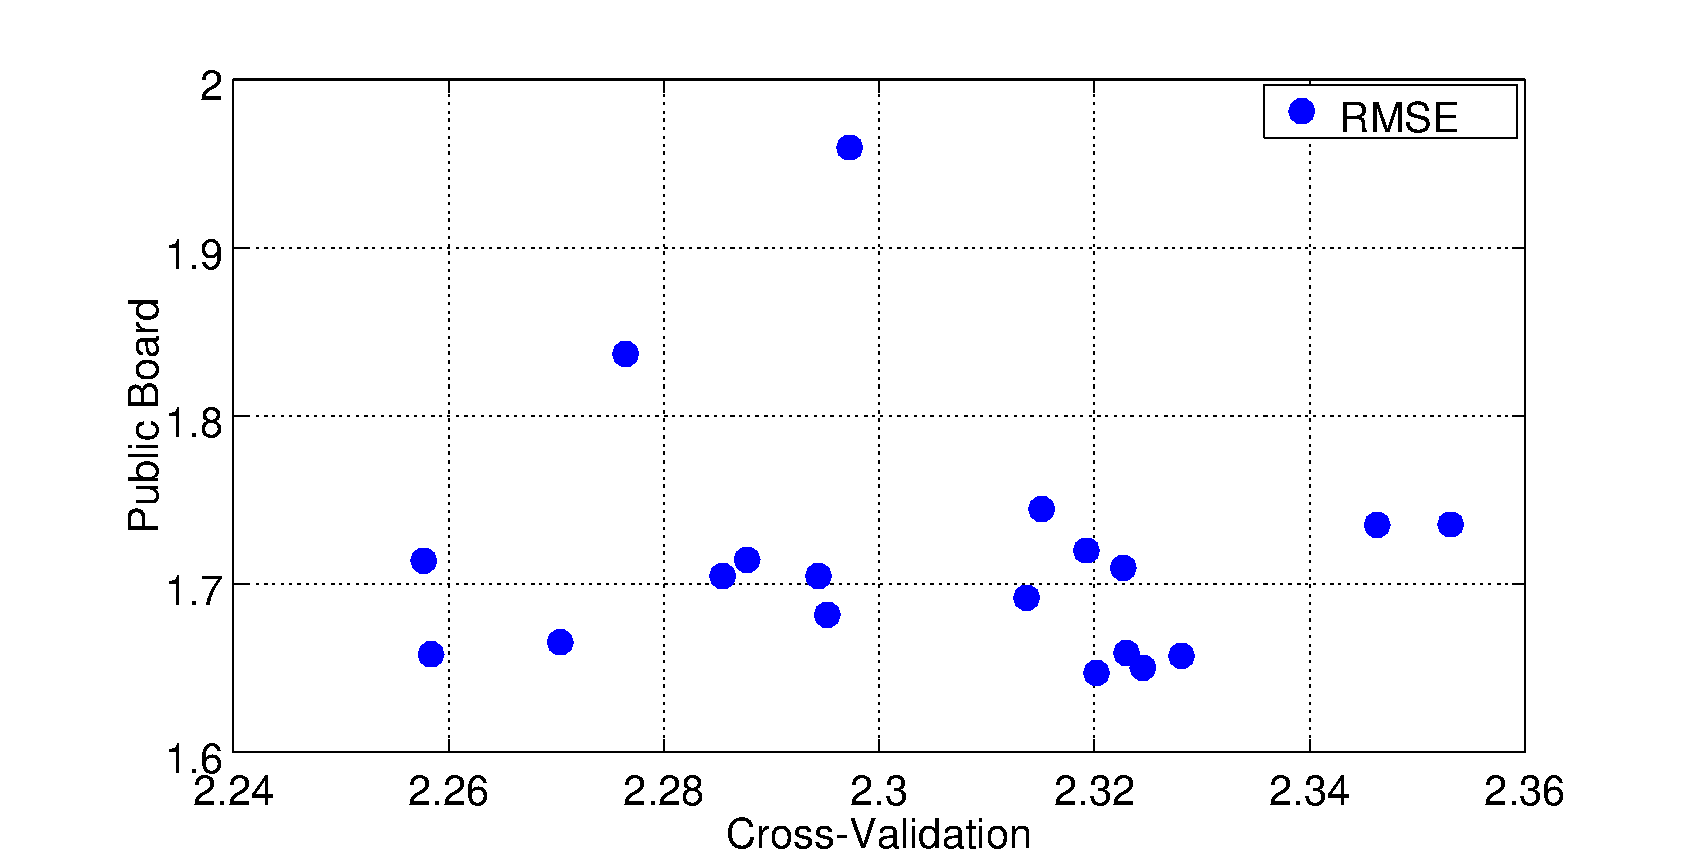
\includegraphics[width=5in]{figs/cv_pb_scores.eps} 
   \caption{RMSE of each submission.}
   \label{fig:cv_lb_error}
\end{figure}


\section{Conclusion}


\end{document}  